\section{Ejercicio 4}

\subsection{Desarrollo}

El ejercicio consiste en programar un scheduler de Round-Robin, para esto utilizaremos las siguientes estructuras: vector de enteros pid$\_$cores, vector de enteros pid$\_$bloqueados, 
vector de enteros quantum$\_$restantes, entero cant$\_$cores, un vector de entero cpu$\_$quantum, Una cola de enteros enEspera.

Cuando creamos el scheduler se nos dan la cantidad de cores(que será cant$\_$cores) y el quantum de cada uno de los cpus(cpu$\_$quantum). Según el enunciado los procesos están agrupados 
en una única cola, de ahí viene enEspera. Como conocemos la cantidad de cores usamos tres estructuras de vectores para, solo teniendo el número del cpu, poder acceder a la 
información de las mismas. pid$\_$bloqueados nos indica si el proceso en cuestión está o no bloqueado(Estos pids no están en enEspera ya que esta corresponde a los
ready), pid$\_$cores nos da el pid del proceso que está corriendo en el cpu y quantum$\_$restantes nos dice cuanto tiempo le queda por ejecutar hasta terminar su tiempo en el 
procesador.

En el programa load en el cual tenemos que poner un proceso en el scheduler lo que haremos será ponerlo en enEspera. En el caso de unblock lo que hacemos es eliminar el pid de 
pid$\_$bloqueados, sabemos que está ahí porque lo añadimos en tick. Por último tenemos el programa tick que se encarga de realizar los procedimientos pertinentes en cada tick de reloj. Tenemos tres casos de motivos:
 
TICK: en el mismo sabemos que ha pasado un tick de reloj y debemos disminuir los quantum que le quedan al procedimiento del cpu. En el caso de que estos terminen en 0 debemos 
plantearnos si debemos desalojar la tarea para poner otra(Si es la IDLE no hacemos nada). De ser el caso, pondremos la tarea actual en la cola enEspera y el próximo elemento
en esta será el nuevo que se hirá ejecutando en este núcleo. Reseteamos el quantum$\_$restantes para que tenga el valor de cpu$\_$quantum del core donde se encuentra. Notece que si no hay más tareas
excepto por la que se estaba ejecutando se volverá a ejecutar la misma.

BLOCK: Si el proceso se va a bloquear añadimos el pid a pid$\_$bloqueados, si existe algún proceso en ready, lo ponemos a ejecutar en ese core. De solo ser un tick en el cual
está bloqueado, solo hacemos lo último(sin añadir a pid$\_$bloqueados).

EXIT: Colocamos en el core la tarea IDLE y si la cola no está vacía, le asignamos la tarea que se encuentre próxima en ella. Después reseteamos los quantum del proceso.


\subsection{Experimentación}

Para poder mostrar el correcto funcionamiento realizamos una serie de experimentos utilizando el lote$\_$simple.tsk, el mismo consiste en tres TaskCPU con distintos parametros.
Los resultados son los siguientes:


\begin{figure}[H]
  \centering
    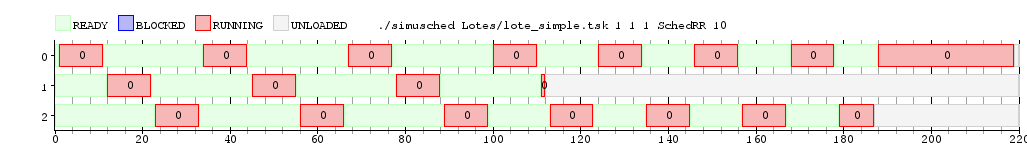
\includegraphics[width=1.1\textwidth]{imagenes/Ej4Experimento1.png}
  \caption{lote$\_$simple.tsk con RR con un core, con quantum de 10}
\end{figure}

\begin{figure}[H]
  \centering
    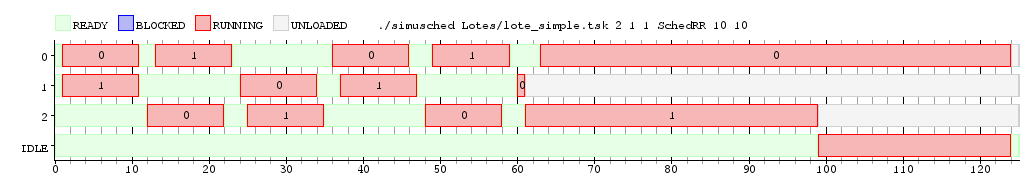
\includegraphics[width=1.1\textwidth]{imagenes/Ej4Experimento2.png}
  \caption{lote$\_$simple.tsk con RR con dos cores y el mismo quantum de 10}
\end{figure}

\begin{figure}[H]
  \centering
    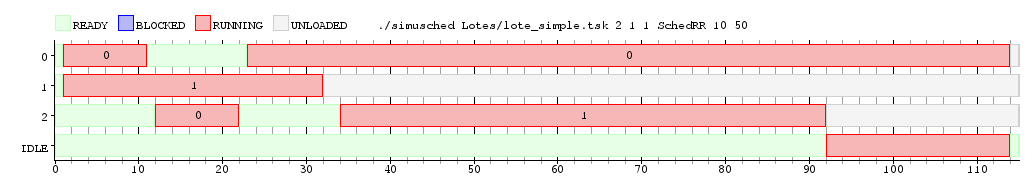
\includegraphics[width=1.1\textwidth]{imagenes/Ej4Experimento3.png}
  \caption{lote$\_$simple.tsk con RR con dos cores, uno con un quantum de 10 y el otro de 50}
\end{figure}

Por los resultados obtenidos podemos ver que, en el primer gráfico, el cpu está ejecutando la primer tarea y pasa a la segunda(sin haber terminado esta última) y luego ejecuta 
por un tiempo para luego pasar a la tercera. Pordemos verlo por lo escalonado del gráfico. Pasando al caso de dos cores, vemos que se repite lo anterior y los núcleos van 
desalojando las tareas para ejecutar otra que este disponible. Por último podemos ver el experimento para mostrar que el scheduler acepta cores con distintos quantums.
Vemos que comienza de forma similar al anterior pero esta vez la segunta tarea(que está ejecutando el segundo core) se encuentra más tiempo en ejecución que la primera
(que está en el primero) y así a lo largo del gráfico.

\begin{figure}[H]
  \centering
    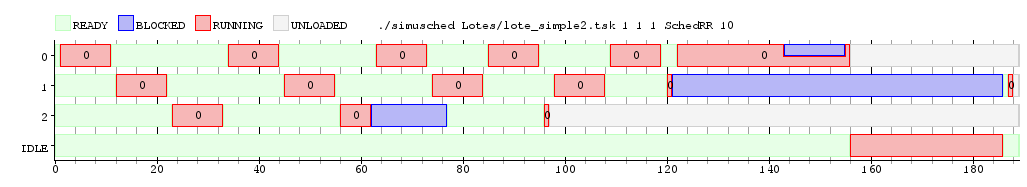
\includegraphics[width=1.1\textwidth]{imagenes/Ej4Experimento4.png}
  \caption{lote$\_$simple2.tsk con RR con un core, con quantum de 10}
\end{figure}

\begin{figure}[H]
  \centering
    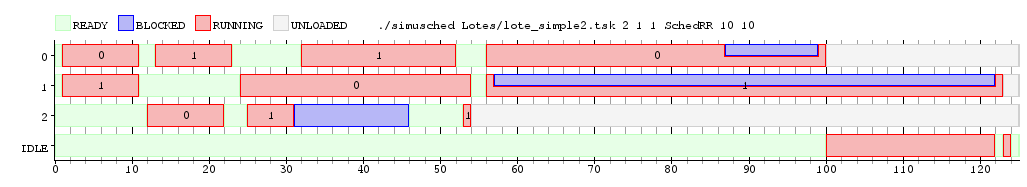
\includegraphics[width=1.1\textwidth]{imagenes/Ej4Experimento5.png}
  \caption{lote$\_$simple2.tsk con RR con dos cores y el mismo quantum de 10}
\end{figure}

\begin{figure}[H]
  \centering
    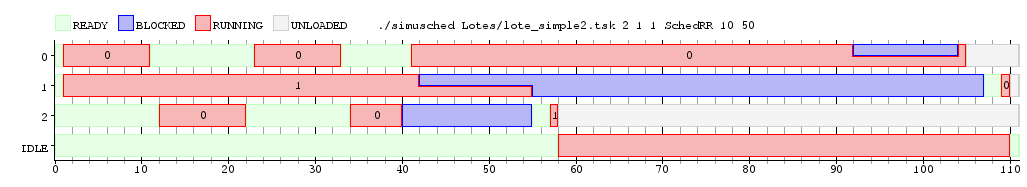
\includegraphics[width=1.1\textwidth]{imagenes/Ej4Experimento6.png}
  \caption{lote$\_$simple2.tsk con RR con dos cores, uno con un quantum de 10 y el otro de 50}
\end{figure}

Repetimos los experimentos solo que con otro lote de tareas(lote_simple2.tsk). Este consiste en llamados bloqueantes usando TaskIO. Lo que pretendemos mostrar es el correcto funcionamiento 
del scheduler cuando hay llamadas bloqueantes. Podemos ver en todos los casos comportamientos similares a los de los anterior tests, pero ahora al momento de bloqueado de 
un proceso el cpu se pone a ejecutar otra tarea disponible, si es que la hay, mientras esa tarea sigue bloqueada. Y con esto mostramos el funcionamiento del scheduler RR.
